\capitulo{4}{Técnicas y herramientas}

\section{Angular}\label{angular}
Angular es un framework de desarrollo de aplicaciones web que es de código abierto y está mantenido por Google, está basado en TypeScript, que es similar a JavaScript y aporta un tipado estático y unas características avanzadas de ES6+, que mejoran la escalabilidad y la capacidad de mantenimiento de los proyectos. 

\begin{center}
  
\includegraphics[width=0.3\textwidth]{img/angular-logo.png}\\
  \small Logotipo de Angular
\end{center}

El principal núcleo que diferencia y da ventaja a Angular respecto a otros frameworks es el concepto de componentes, que son unidades que combinan html, typescript y css. Cada componente representa una de las partes que se ven en la interfaz de usuario y se pueden anidar unos con otros formando jerarquías que definirán la estructura final que tendrá la aplicación. Estos componentes se agrupan en modulos, que permiten organizar el código en diferentes funcionalidades y admitir de esa forma la carga perezosa (lazy loading) para que se cargue solo la informacion esencial en cada ventana y se mejore el rendimiento.

Para hacer la gestión de la comunicación entre componentes y servicios, Angular tiene un sistema que se llama inyección de depencencias, con el que se registran en los injectors o contenedores los servicios que sirven para acceder a datos.

Angular también incluye un enrutador (Router) que permite definir rutas y navegacion dentro de la aplicacion web, gestionando los parámetros, posibles rutas hijas y los guards que controlan el acceso a apartados de la aplicacion segun los permisos que se quieran dar. Junto con angular cli, ofrece un ecosistema muy maduro. lo que lo convierte en una opción sólida para construir aplicaciones web robustas, mantenibles y de gran escala.

\section{Angular CLI}\label{angular-cli}
Es una herramienta de línea de comandos que acelera la creación, compilación y el despliegue de los proyectos, de manera que permite aplicar mejores prácticas de forma automática.

\begin{center}
  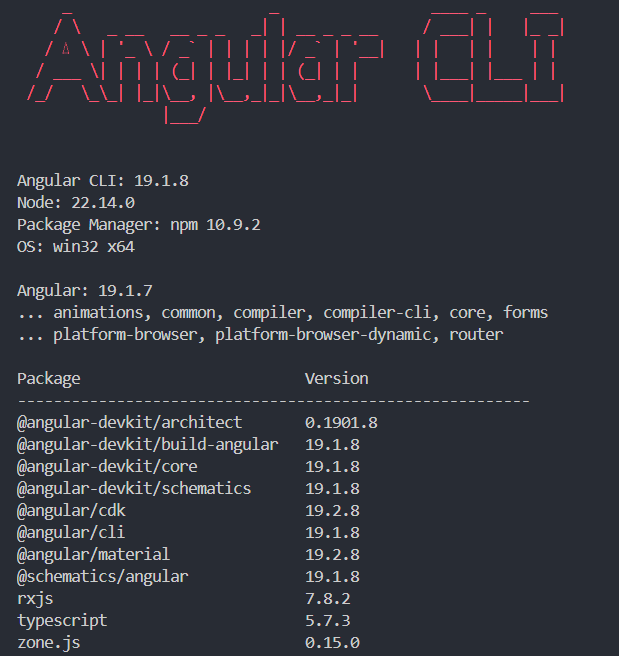
\includegraphics[width=0.7\textwidth]{img/angular-cli.png}\\
  \small Angular CLI
\end{center}

\section{Control de versiones}\label{control-versiones}
Git es un sistema de control de versiones distribuido que está diseñado para poder gestionar el historial de cambios en proyectos de software.
\href{https://git-scm.com/}{Git}

\begin{center}
  
\includegraphics[width=0.3\textwidth]{img/git-logo.png}\\
  \small Logotipo de Git
\end{center}

\section{Github}\label{github}
\href{https://github.com/}{Github} es una plataforma en la nube que permite subir proyectos de software que utilizan el sistema de control de versiones Git. 

\begin{center}
  
\includegraphics[width=0.2\textwidth]{img/github-logo.png}\\
  \small Logotipo de GitHub
\end{center}

Subir código a un repositorio de GitHub implica los siguientes pasos básicos:

\subsection{Inicializar o clonar un repositorio Git}
Dentro de la carpeta de un proyecto, permite crear un repositorio local.
Cuando hay un proyecto existente, permite clonarlo para traer una copia local.

\subsection{Gestionar cambios con commits}
Después de crear o modificar archivos, se añaden al área de preparación (staging area) y se registran los cambios con un commit.

\subsection{Conectar el repositorio local con GitHub}
Si no se ha clonado, se puede añadir una URL remota en la que subir el código.

\subsection{Enviar (push) cambios al repositorio en GitHub}
Para subir la rama principal

\subsection{Trabajo colaborativo y ramas}
Ramas (`branches`): consiste en crear nuevas líneas de desarrollo y cambiarse a ellas.
Pull requests (PR): en la interfaz web de GitHub, proponer que tu rama se fusione (“merge”) en la rama principal tras revisión de código.

\subsection{Beneficios de usar GitHub}
Historial de versiones: permite regresar a estados anteriores del proyecto.
Colaboración: múltiples desarrolladores pueden trabajar simultáneamente sin pisarse cambios.
Visibilidad: proyectos open-source se comparten con la comunidad; repositorios privados para código interno.

Con lo que, subir los códigos a GitHub no consiste solamente en copiar y pegar ficheros, sino en aprovechar todo un ecosistema de control de versiones, asegurando que cada cambio quede documentado, pueda revisarse y desplegarse siguiendo buenas prácticas de desarrollo.


\section{HeidiSQL con MySQL}\label{heidi-sql}
HeidiSQL es un cliente gráfico gratuito para Windows diseñado principalmente para gestionar bases de datos MySQL, MariaDB y otros motores compatibles (como por ejemplo PostgreSQL o Microsoft SQL Server). 

\begin{center}
  
\includegraphics[width=0.25\textwidth]{img/heidi-logo.png}\\
  \small Logotipo de HeidiSQL
\end{center}

Al usarlo con MySQL, HeidiSQL ofrece una interfaz intuitiva que permite:
Conectarse y navegar por servidores MySQL mediante un administrador de sesiones, donde puedes guardar múltiples configuraciones de conexión (host, puerto, usuario, contraseña, etc.).

Visualizar y editar estructuras de bases de datos, tablas, vistas y procedimientos almacenados con un explorador de objetos que muestra de forma jerárquica todos los elementos.
Ejecutar consultas SQL en un editor con resaltado de sintaxis, autocompletado y pestañas múltiples para trabajar en varios scripts a la vez.

Importar y exportar datos de forma sencilla: puedes volcar estructuras y datos a archivos SQL, CSV, XML o incluso sincronizar bases de datos entre servidores con su herramienta de comparación.

Monitorear la actividad del servidor MySQL (procesos activos, status variables) y obtener estadísticas básicas de rendimiento.

\begin{center}
  
\includegraphics[width=0.4\textwidth]{img/mysql-logo.png}\\
  \small Logotipo de MySQL
\end{center}

HeidiSQL es muy útil cuando se necesita un acceso rápido y eficiente a bases de datos MySQL sin complicaciones de configuraciones avanzadas ni licencias de pago.

\section{Google AI Studio e integración en .NET}\label{google-ai-studio}
Google AI Studio (antes conocido como Vertex AI Workbench) es la plataforma de Google Cloud que unifica herramientas para el desarrollo, entrenamiento, despliegue y monitorización de modelos de inteligencia artificial y machine learning. 

\begin{center}
  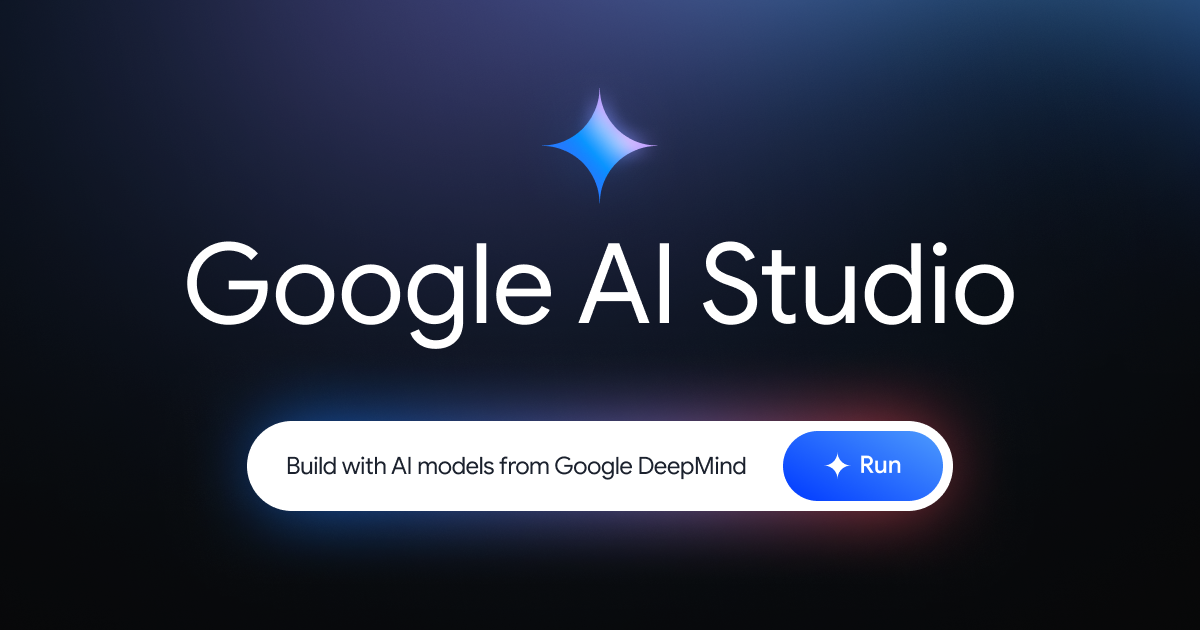
\includegraphics[width=0.5\textwidth]{img/ai-studio-logo.png}\\
  \small Logotipo de Google AI Studio
\end{center}

\subsection{Integración con Google AI Studio en .NET}

La aplicación .NET se conecta a Google AI Studio empleando las librerías oficiales de Google Cloud para .NET, lo que permite aprovechar capacidades avanzadas de IA directamente desde nuestro entorno de desarrollo. El proceso de integración consta de cuatro pasos clave:

\begin{enumerate}
  \item \textbf{Instalación}: añadir el paquete NuGet  
    \texttt{Google.Cloud.AIPlatform.V1} al proyecto.
  \item \textbf{Autenticación}: configurar y utilizar una cuenta de servicio  
    cuyas credenciales se cargan en las variables de entorno.
  \item \textbf{Invocación de la API}: llamar a los métodos de la biblioteca  
    para entrenar, evaluar o desplegar modelos de Machine Learning.
  \item \textbf{Gestión y monitorización}: para procesar las respuestas de la API y supervisar métricas y registros desde el propio código .NET.
\end{enumerate}

Gracias a esta integración, se pueden automatizar tareas de aprendizaje automático sin abandonar todo el ecosistema de .NET, manteniendo una experiencia de desarrollo coherente.
